\documentclass[tikz,border=2mm]{standalone}
\usepackage[T1]{fontenc}
\usepackage[swedish,english]{babel}
\usepackage{tikz}
\usetikzlibrary{arrows,positioning}
\usepackage{pgfplots}
\usepackage{amsmath,mathtools}
\usepgfplotslibrary{fillbetween}
\begin{document}
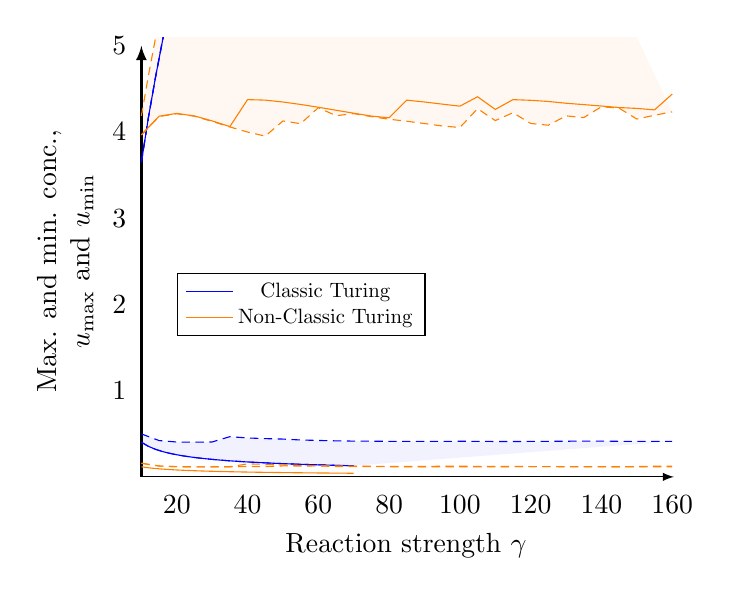
\begin{tikzpicture}
\begin{axis}[
    %hide axis,
    %axis lines* = left,
    %axis lines=left, xtick=\empty, ytick=\empty.
    axis line style={draw=none},
    tick style={draw=none},
    xticklabel style={yshift=-0.1mm},
    xmin = 8.5,
   xmax = 161,
   ymin = -0.1,
    ymax = 5.1,
    %grid=both,
    %xtick = {1,0.95,...,0.6},
    ytick = {1,...,6},    
    %xticklabels = {{zero},$\alpha$,$\varphi$},
   %xlabel style={at={(axis cs:0.61,7)},anchor=east,align=center},
    %ylabel style={at={(axis cs:1.00,35)},anchor=north,rotate=0},
	xlabel = {Reaction strength $\gamma$},
        ylabel = {Max. and min. conc.,\\ $u_{\max}$ and $u_{\min}$},
        ylabel style = {align=center},
    legend style={at={(axis cs:20,2.0)},anchor=west,cells={align=center},nodes={scale=0.75}},
    %x dir=reverse
    %legend entries = {Decreasing the inactivation rate $k_{-2}$}
]
%-------------------------------------------------------------------------------------------------
% AXES
\draw[->,-latex, thick] (axis cs: 10,0) -- (axis cs: 10,5.0); % y-axis
\draw[->,-latex] (axis cs: 10,0) -- (axis cs: 160.5,0); % x-axis
%-------------------------------------------------------------------------------------------------
%-------------------------------------------------------------------------------------------------
% Classical 
%-------------------------------------------------------------------------------------------------
\addplot[forget plot,densely dashed,color=blue,name path=UpuMaxClassical] coordinates {
		(10.0000	,	3.6544	)
		(12.0000	,	4.1770	)
		(14.0000	,	4.6427	)
		(16.0000	,	5.0724	)
		(18.0000	,	5.4677	)
		(20.0000	,	5.8404	)
		(22.0000	,	6.1886	)
		(24.0000	,	6.5217	)
		(26.0000	,	6.8394	)
		(28.0000	,	7.1372	)
		(30.0000	,	7.4308	)
		(32.0000	,	7.7136	)
		(34.0000	,	7.9777	)
		(36.0000	,	8.2420	)
		(38.0000	,	8.5047	)
		(40.0000	,	8.7328	)
		(42.0000	,	8.9718	)
		(44.0000	,	9.2079	)
		(46.0000	,	9.4224	)
		(48.0000	,	9.6469	)
		(50.0000	,	9.8536	)
		(52.0000	,	10.0608	)
		(54.0000	,	10.2724	)
		(56.0000	,	10.4570	)
		(58.0000	,	10.6565	)
		(60.0000	,	10.8357	)
		(62.0000	,	11.0273	)
		(64.0000	,	11.2129	)
		(66.0000	,	11.4008	)
		(68.0000	,	11.5569	)
		(70.0000	,	11.7288	)
};

\addplot[forget plot,color=blue] coordinates {
		(10.0000	,	3.6501	)
		(12.0000	,	4.1733	)
		(14.0000	,	4.6393	)
		(16.0000	,	5.0664	)
		(18.0000	,	5.4618	)
		(20.0000	,	5.8354	)
		(22.0000	,	6.1846	)
		(24.0000	,	6.5148	)
		(26.0000	,	6.8322	)
		(28.0000	,	7.1297	)
		(30.0000	,	7.4201	)
		(32.0000	,	7.7006	)
		(34.0000	,	7.9744	)
		(36.0000	,	8.2273	)
		(38.0000	,	8.4819	)
		(40.0000	,	8.7187	)
		(42.0000	,	8.9565	)
		(44.0000	,	9.1862	)
		(46.0000	,	9.4119	)
		(48.0000	,	9.6292	)
		(50.0000	,	9.8420	)
		(52.0000	,	10.0430	)
		(54.0000	,	10.2475	)
		(56.0000	,	10.4441	)
		(58.0000	,	10.6346	)
		(60.0000	,	10.8235	)
		(62.0000	,	11.0092	)
		(64.0000	,	11.1881	)
		(66.0000	,	11.3625	)
		(68.0000	,	11.5291	)
		(70.0000	,	11.7093	)
};

\addplot[forget plot,densely dashed,color=blue,name path=DownuMaxClassical] coordinates {
		(10.0000	,	3.6475	)
		(12.0000	,	4.1694	)
		(14.0000	,	4.6316	)
		(16.0000	,	5.0624	)
		(18.0000	,	5.4572	)
		(20.0000	,	5.8282	)
		(22.0000	,	6.1781	)
		(24.0000	,	6.5063	)
		(26.0000	,	6.8264	)
		(28.0000	,	7.1222	)
		(30.0000	,	7.4115	)
		(32.0000	,	7.6902	)
		(34.0000	,	7.9597	)
		(36.0000	,	8.2160	)
		(38.0000	,	8.4758	)
		(40.0000	,	8.7102	)
		(42.0000	,	8.9413	)
		(44.0000	,	9.1679	)
		(46.0000	,	9.3962	)
		(48.0000	,	9.6101	)
		(50.0000	,	9.8220	)
		(52.0000	,	10.0284	)
		(54.0000	,	10.2237	)
		(56.0000	,	10.4223	)
		(58.0000	,	10.6012	)
		(60.0000	,	10.7954	)
		(62.0000	,	10.9888	)
		(64.0000	,	11.1594	)
		(66.0000	,	11.3399	)
		(68.0000	,	11.5134	)
		(70.0000	,	11.6838	)
};
\addplot[blue!50,opacity=0.1,forget plot] fill between[of=UpuMaxClassical and DownuMaxClassical];

\addplot[forget plot,densely dashed,color=blue,name path=UpuMinClassical] coordinates {
		(10.0000	,	0.4981	)
		(15.0000	,	0.4211	)
		(20.0000	,	0.4041	)
		(25.0000	,	0.4020	)
		(30.0000	,	0.4050	)
		(35.0000	,	0.4664	)
		(40.0000	,	0.4512	)
		(45.0000	,	0.4436	)
		(50.0000	,	0.4384	)
		(55.0000	,	0.4278	)
		(60.0000	,	0.4224	)
		(65.0000	,	0.4177	)
		(70.0000	,	0.4148	)
		(75.0000	,	0.4137	)
		(80.0000	,	0.4120	)
		(85.0000	,	0.4116	)
		(90.0000	,	0.4112	)
		(95.0000	,	0.4111	)
		(100.0000	,	0.4127	)
		(105.0000	,	0.4121	)
		(110.0000	,	0.4105	)
		(115.0000	,	0.4099	)
		(120.0000	,	0.4111	)
		(125.0000	,	0.4124	)
		(130.0000	,	0.4135	)
		(135.0000	,	0.4145	)
		(140.0000	,	0.4154	)
		(145.0000	,	0.4122	)
		(150.0000	,	0.4117	)
		(155.0000	,	0.4118	)
		(160.0000	,	0.4117	)
};

\addplot[color=blue] coordinates {
		(10.0000	,	0.4019	)
		(12.0000	,	0.3537	)
		(14.0000	,	0.3195	)
		(16.0000	,	0.2935	)
		(18.0000	,	0.2732	)
		(20.0000	,	0.2563	)
		(22.0000	,	0.2423	)
		(24.0000	,	0.2303	)
		(26.0000	,	0.2200	)
		(28.0000	,	0.2109	)
		(30.0000	,	0.2029	)
		(32.0000	,	0.1956	)
		(34.0000	,	0.1891	)
		(36.0000	,	0.1833	)
		(38.0000	,	0.1779	)
		(40.0000	,	0.1730	)
		(42.0000	,	0.1686	)
		(44.0000	,	0.1644	)
		(46.0000	,	0.1605	)
		(48.0000	,	0.1568	)
		(50.0000	,	0.1535	)
		(52.0000	,	0.1503	)
		(54.0000	,	0.1473	)
		(56.0000	,	0.1445	)
		(58.0000	,	0.1419	)
		(60.0000	,	0.1394	)
		(62.0000	,	0.1370	)
		(64.0000	,	0.1347	)
		(66.0000	,	0.1326	)
		(68.0000	,	0.1305	)
		(70.0000	,	0.1286	)
};

\addplot[forget plot,densely dashed,color=blue,name path=DownuMinClassical] coordinates {
		(10.0000	,	0.4009	)
		(12.0000	,	0.3529	)
		(14.0000	,	0.3190	)
		(16.0000	,	0.2931	)
		(18.0000	,	0.2728	)
		(20.0000	,	0.2560	)
		(22.0000	,	0.2421	)
		(24.0000	,	0.2301	)
		(26.0000	,	0.2198	)
		(28.0000	,	0.2108	)
		(30.0000	,	0.2027	)
		(32.0000	,	0.1955	)
		(34.0000	,	0.1890	)
		(36.0000	,	0.1831	)
		(38.0000	,	0.1778	)
		(40.0000	,	0.1729	)
		(42.0000	,	0.1684	)
		(44.0000	,	0.1642	)
		(46.0000	,	0.1603	)
		(48.0000	,	0.1567	)
		(50.0000	,	0.1533	)
		(52.0000	,	0.1501	)
		(54.0000	,	0.1472	)
		(56.0000	,	0.1444	)
		(58.0000	,	0.1418	)
		(60.0000	,	0.1393	)
		(62.0000	,	0.1369	)
		(64.0000	,	0.1346	)
		(66.0000	,	0.1325	)
		(68.0000	,	0.1305	)
		(70.0000	,	0.1285	)
};
\addplot[blue!50,opacity=0.1,forget plot] fill between[of=UpuMinClassical and DownuMinClassical];

\addlegendentry{Classic Turing}% Add to legend
%-------------------------------------------------------------------------------------------------
% Non-classical
%-------------------------------------------------------------------------------------------------
\addplot[forget plot,densely dashed,color=orange,name path=UpuMaxNonClassical] coordinates {
		(10.0000	,	4.1878	)
		(12.0000	,	4.6571	)
		(14.0000	,	5.0925	)
		(16.0000	,	5.4905	)
		(18.0000	,	5.8700	)
		(20.0000	,	6.2289	)
		(22.0000	,	6.5641	)
		(24.0000	,	6.8880	)
		(26.0000	,	7.1961	)
		(28.0000	,	7.4935	)
		(30.0000	,	7.7764	)
		(32.0000	,	8.0500	)
		(34.0000	,	8.3158	)
		(36.0000	,	8.5724	)
		(38.0000	,	8.8221	)
		(40.0000	,	9.0575	)
		(42.0000	,	9.2867	)
		(44.0000	,	9.5157	)
		(46.0000	,	9.7485	)
		(48.0000	,	9.9577	)
		(50.0000	,	10.1675	)
		(52.0000	,	10.3692	)
		(54.0000	,	10.5683	)
		(56.0000	,	10.7639	)
		(58.0000	,	10.9618	)
		(60.0000	,	11.1531	)
		(62.0000	,	11.3225	)
		(64.0000	,	11.5024	)
		(66.0000	,	11.6954	)
		(68.0000	,	11.8583	)
		(70.0000	,	12.0386	)
};

\addplot[forget plot,color=orange] coordinates {
		(10.0000	,	3.9685	)
		(15.0000	,	4.1835	)
		(20.0000	,	4.2159	)
		(25.0000	,	4.1861	)
		(30.0000	,	4.1289	)
		(35.0000	,	4.0629	)
		(40.0000	,	4.3758	)
		(45.0000	,	4.3700	)
		(50.0000	,	4.3481	)
		(55.0000	,	4.3198	)
		(60.0000	,	4.2874	)
		(65.0000	,	4.2526	)
		(70.0000	,	4.2183	)
		(75.0000	,	4.1845	)
		(80.0000	,	4.1653	)
		(85.0000	,	4.3695	)
		(90.0000	,	4.3482	)
		(95.0000	,	4.3237	)
		(100.0000	,	4.2999	)
		(105.0000	,	4.4090	)
		(110.0000	,	4.2621	)
		(115.0000	,	4.3756	)
		(120.0000	,	4.3681	)
		(125.0000	,	4.3544	)
		(130.0000	,	4.3340	)
		(135.0000	,	4.3179	)
		(140.0000	,	4.3017	)
		(145.0000	,	4.2838	)
		(150.0000	,	4.2741	)
		(155.0000	,	4.2566	)
		(160.0000	,	4.4399	)
};

\addplot[forget plot,densely dashed,color=orange,name path=DownuMaxNonClassical] coordinates {
		(10.0000	,	3.9647	)
		(15.0000	,	4.1803	)
		(20.0000	,	4.2117	)
		(25.0000	,	4.1832	)
		(30.0000	,	4.1226	)
		(35.0000	,	4.0588	)
		(40.0000	,	3.9997	)
		(45.0000	,	3.9520	)
		(50.0000	,	4.1284	)
		(55.0000	,	4.0966	)
		(60.0000	,	4.2823	)
		(65.0000	,	4.1895	)
		(70.0000	,	4.2133	)
		(75.0000	,	4.1786	)
		(80.0000	,	4.1481	)
		(85.0000	,	4.1251	)
		(90.0000	,	4.0983	)
		(95.0000	,	4.0699	)
		(100.0000	,	4.0527	)
		(105.0000	,	4.2706	)
		(110.0000	,	4.1328	)
		(115.0000	,	4.2239	)
		(120.0000	,	4.0994	)
		(125.0000	,	4.0789	)
		(130.0000	,	4.1873	)
		(135.0000	,	4.1674	)
		(140.0000	,	4.2932	)
		(145.0000	,	4.2770	)
		(150.0000	,	4.1506	)
		(155.0000	,	4.1945	)
		(160.0000	,	4.2345	)
};
\addplot[orange!50,opacity=0.1,forget plot] fill between[of=UpuMaxNonClassical and DownuMaxNonClassical];

\addplot[forget plot,densely dashed,color=orange,name path=UpuMinNonClassical] coordinates {
		(10.0000	,	0.1581	)
		(15.0000	,	0.1260	)
		(20.0000	,	0.1183	)
		(25.0000	,	0.1165	)
		(30.0000	,	0.1167	)
		(35.0000	,	0.1176	)
		(40.0000	,	0.1504	)
		(45.0000	,	0.1458	)
		(50.0000	,	0.1381	)
		(55.0000	,	0.1333	)
		(60.0000	,	0.1294	)
		(65.0000	,	0.1269	)
		(70.0000	,	0.1249	)
		(75.0000	,	0.1227	)
		(80.0000	,	0.1215	)
		(85.0000	,	0.1206	)
		(90.0000	,	0.1200	)
		(95.0000	,	0.1240	)
		(100.0000	,	0.1230	)
		(105.0000	,	0.1221	)
		(110.0000	,	0.1210	)
		(115.0000	,	0.1203	)
		(120.0000	,	0.1195	)
		(125.0000	,	0.1190	)
		(130.0000	,	0.1187	)
		(135.0000	,	0.1183	)
		(140.0000	,	0.1180	)
		(145.0000	,	0.1178	)
		(150.0000	,	0.1194	)
		(155.0000	,	0.1229	)
		(160.0000	,	0.1241	)
};

\addplot[color=orange] coordinates {
		(10.0000	,	0.1164	)
		(12.0000	,	0.1053	)
		(14.0000	,	0.0969	)
		(16.0000	,	0.0902	)
		(18.0000	,	0.0847	)
		(20.0000	,	0.0800	)
		(22.0000	,	0.0761	)
		(24.0000	,	0.0727	)
		(26.0000	,	0.0697	)
		(28.0000	,	0.0670	)
		(30.0000	,	0.0647	)
		(32.0000	,	0.0625	)
		(34.0000	,	0.0606	)
		(36.0000	,	0.0588	)
		(38.0000	,	0.0572	)
		(40.0000	,	0.0557	)
		(42.0000	,	0.0543	)
		(44.0000	,	0.0530	)
		(46.0000	,	0.0519	)
		(48.0000	,	0.0507	)
		(50.0000	,	0.0497	)
		(52.0000	,	0.0487	)
		(54.0000	,	0.0478	)
		(56.0000	,	0.0469	)
		(58.0000	,	0.0461	)
		(60.0000	,	0.0453	)
		(62.0000	,	0.0446	)
		(64.0000	,	0.0439	)
		(66.0000	,	0.0432	)
		(68.0000	,	0.0426	)
		(70.0000	,	0.0420	)
};

\addplot[forget plot,densely dashed,color=orange,name path=DownuMinNonClassical] coordinates {
		(10.0000	,	0.1572	)
		(15.0000	,	0.1257	)
		(20.0000	,	0.1180	)
		(25.0000	,	0.1164	)
		(30.0000	,	0.1166	)
		(35.0000	,	0.1174	)
		(40.0000	,	0.1185	)
		(45.0000	,	0.1195	)
		(50.0000	,	0.1271	)
		(55.0000	,	0.1256	)
		(60.0000	,	0.1273	)
		(65.0000	,	0.1199	)
		(70.0000	,	0.1210	)
		(75.0000	,	0.1185	)
		(80.0000	,	0.1179	)
		(85.0000	,	0.1176	)
		(90.0000	,	0.1175	)
		(95.0000	,	0.1176	)
		(100.0000	,	0.1176	)
		(105.0000	,	0.1177	)
		(110.0000	,	0.1178	)
		(115.0000	,	0.1180	)
		(120.0000	,	0.1182	)
		(125.0000	,	0.1183	)
		(130.0000	,	0.1177	)
		(135.0000	,	0.1175	)
		(140.0000	,	0.1174	)
		(145.0000	,	0.1172	)
		(150.0000	,	0.1172	)
		(155.0000	,	0.1171	)
		(160.0000	,	0.1170	)
};
\addplot[orange!50,opacity=0.1,forget plot] fill between[of=UpuMinNonClassical and DownuMinNonClassical];

\addlegendentry{Non-Classic Turing}% Add to legend
\end{axis}

\end{tikzpicture}



\end{document}
